\documentclass[journal]{IEEEtran}
\usepackage{float}
\usepackage[export]{adjustbox}
\usepackage{graphicx}
\usepackage{caption}
\usepackage{amsmath}
\usepackage{algorithmic}
\usepackage{listings}
\usepackage{amsmath}
\lstset{
  frame=single,
  language=C,
  basicstyle=\small,
}
\ifCLASSOPTIONcompsoc
 \usepackage[caption=false,font=normalsize,labelfont=sf,textfont=sf]{subfig}
\else
 \usepackage[caption=false,font=footnotesize]{subfig}
\fi
\usepackage{siunitx}
\usepackage{biblatex}
\DeclareMathOperator*{\argmin}{\arg\min} 
\addbibresource{bibliography.bib}




\begin{document}
\title{Laboratory Assignment 4 - 3D Reconstruction}
\author{João Pedro Castilho, 2017263424\\
        Gonçalo Arsénio, 2017246034}
\maketitle
\IEEEpeerreviewmaketitle
\section{Introdução}
Neste trabalho é nos pedido para recuperar a estrutura 3D de um ambiente, juntamente com a posição da câmara, tendo apenas duas imagens 2D do mesmo ambiente. Para tal, vão ser usados dois algoritmos:
\begin{enumerate}
    \item Sparse Reconstruction
    \item Dense Reconstruction
\end{enumerate}
\par Técnicas de reconstrução 3D são usadas em vários campos da ciência e engenharia como na medicina, mapeamento feito por robôs moveis ou realidade aumentada.
\par No relatório vamos explicar a nossa implementação dos três algoritmos propostos e apresentar os resultados obtidos.
\par As imagens utilizadas para fazer a reconstrução 3D foram as seguintes.
\begin{figure}[H]
        \centering
        \subfloat[Imagem da Esquerda]{\label{fig:1}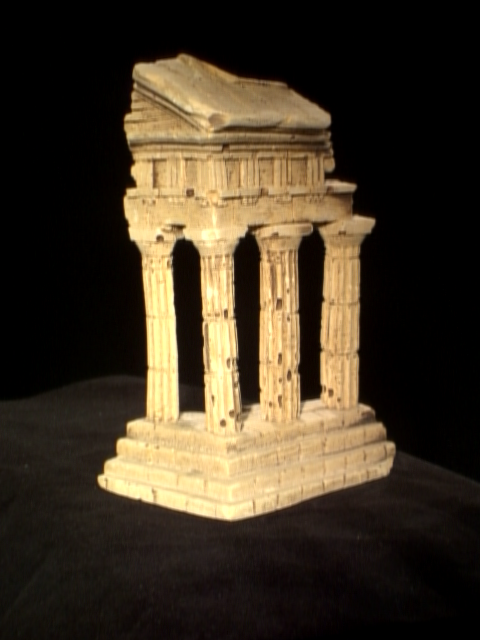
\includegraphics[width=1.2in]{Images/im1.png}}
        \qquad
        \subfloat[Imagem da Direita]{\label{fig:2}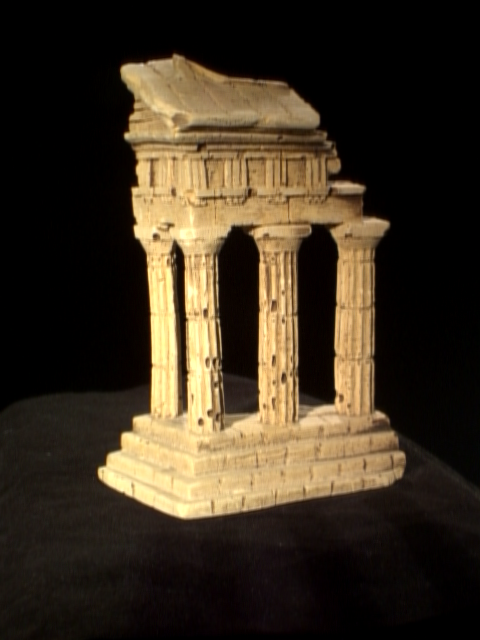
\includegraphics[width=1.2in]{Images/im2.png}}
        \caption{Imagens usadas para a reconstrução 3D}
        \label{fig:3}
\end{figure}
\section{Sparse Reconstruction}
\subsection*{Matriz Fundamental}
\par A matriz fundamental correlaciona duas imagens do mesmo cenário, onde os pontos de uma das imagens podem ser projetados noutra. A restrição entre estes ponto pode ser referida como restrição epipolar.
\par Para fazer o cálculo desta matriz foi usada a função \textit{computeF} que vai ter como parâmetros de entrada os pontos na imagem da direita e os mesmos pontos na imagem da esquerda.
\par Primeiramente vamos ter de normalizar os pontos fornecidos, consequentemente foi utilizada a função \textit{normalization} desenvolvida no trabalho anterior.
\par Após a normalização dos pontos vamos calcular a matriz \textit{A} dada por:

\begin{equation}
    \begin{bmatrix}
    x_1x_1' & y1x_1' & x_1' & x_1y_1' & y_1y_1' & y_1' & x_1 & y_1 & 1 \\
    x_2x_2' & y2x_2' & x_2' & x_2y_2' & y_2y_2' & y_2' & x_2 & y_2 & 1 \\
            &        &      &         &    \vdots     &      &     &     &
    \end{bmatrix}
\end{equation}
sendo $(x,y)$ os pontos da primeira imagem e os $(x',y')$ os da segunda.

\par Obtendo esta matriz vamos ter de fazer a sua decomposição em valores singulares, $A = UDV^T$, sendo \textit{F} a última coluna da matriz \textit{V}. No entanto, a matriz \textit{A} tem rank 9 e nós queremos que a nossa solução tenha rank 2, como tal vamos ter de forçar isso, decompondo essa matriz \textit{F} em valores singulares, $F = UDV^T$, e substituir o menor valor singular da diagonal da matriz \textit{D} por zero, ficando:
\begin{equation}
    F = UD´V^T
\end{equation}
\par Para otimizar a nossa solução foi utilizada a função \textit{refineF} fornecida pelo professor. Fazendo a otimização fica apenas a faltar a desnormalização da matriz fundamental:
\begin{equation}
    F_d = T_r^TFT_l
\end{equation}
sendo $T_r$ e $T_l$ as matrizes de transformação obtidas após a desnormalização dos pontos das respectivas imagens fornecidas.
\par As linhas epipolares obtidas através desta matriz podem ser visualizadas abaixo.
\begin{figure}[H]
        \centering
        \subfloat[Pontos seleccionados]{\label{fig:4}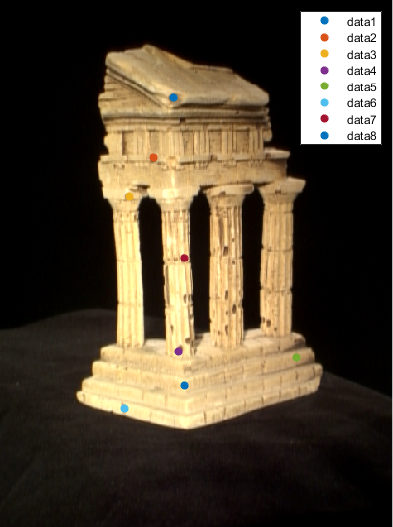
\includegraphics[width=1.2in]{Images/Epi1.png}}
        \qquad
        \subfloat[Linhas obtidas]{\label{fig:5}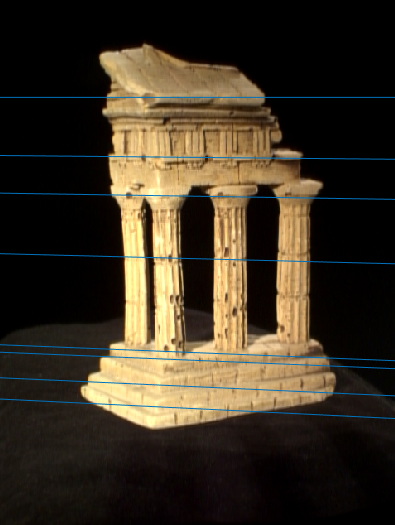
\includegraphics[width=1.2in]{Images/Epi2.png}}
        \caption{Linhas Epipolares}
        \label{fig:6}
\end{figure}

\subsection*{Correspondências Epipolares}
\par Agora que temos a matriz fundamental \textit{F} podemos usa-la para fazer a correspondência entre pontos característicos entre as duas imagens apenas percorrendo as linhas epipolares correspondentes a esses pontos. Este método de obter correspondências entre duas imagens apresenta uma vantagem em relação ao trabalho desenvolvido no Lab 2, porque usando as linhas epipolares não precisamos de percorrer a imagem toda à procura de correspondências.
\par O primeiro passo do algoritmo é calcular os parâmetros da linha epipolar correspondente a um ponto $(x,y)$. Sendo a linha epipolar parametrizada da forma:
\begin{equation}
   l\Rightarrow ax+by-c=0
\end{equation}
a linha epipolar \textit{l} vai ser igual a:
\begin{equation}
    l=F\begin{bmatrix}
    x\\y\\1
    \end{bmatrix}
\end{equation}
a linha \textit{l} é depois normalizada de acordo com a sua norma, $|l|=\sqrt{a^2+b^2}$.
\par Agora que temos a parametrização das linhas epipolares correspondentes aos  pontos já conseguimos fazer as correspondências através das linhas epipolares. O descritor usado foi o Simple com uma janela de 25 pixeis e o critério de matching usado foi o \textit{ratio test}.
\begin{lstlisting}[
  caption=Correspondências epipolares,
  label=lst1:mxm,
  basicstyle=\tiny
]
%Convert the image to grayscale
im1=double(rgb2gray(im1));

%Get the descriptors for all the points in img1
[DesciptorsImg1]=SimpleFeatureDescriptor(im1,pts1,5);
pts2=[];

for n=1:size(l,1)  
    %Gets all the points from the epipolar line
    for x=1:size(im1,2)
        p2(x,2) = -(l(n,1) * x + l(n,3))/l(n,2);
        p2(x,1)=x;
    end
    
    %Gets all the descriptors for the points in the line
    [DesciptorsImg2]=SimpleFeatureDescriptor(im2,p2,5); 
    
    %Matches the two descriptors
    [Match,NoMatch]=RatioFeatureMatcher(DesciptorsImg1(n,:),DesciptorsImg2,10); 
    
    pts2=[pts2;Match(2) floor(p2(Match(2),2))];
end
\end{lstlisting}

\begin{figure}[H]
        \centering
        \subfloat[Pontos na imagem da esquerda]{\label{fig:7}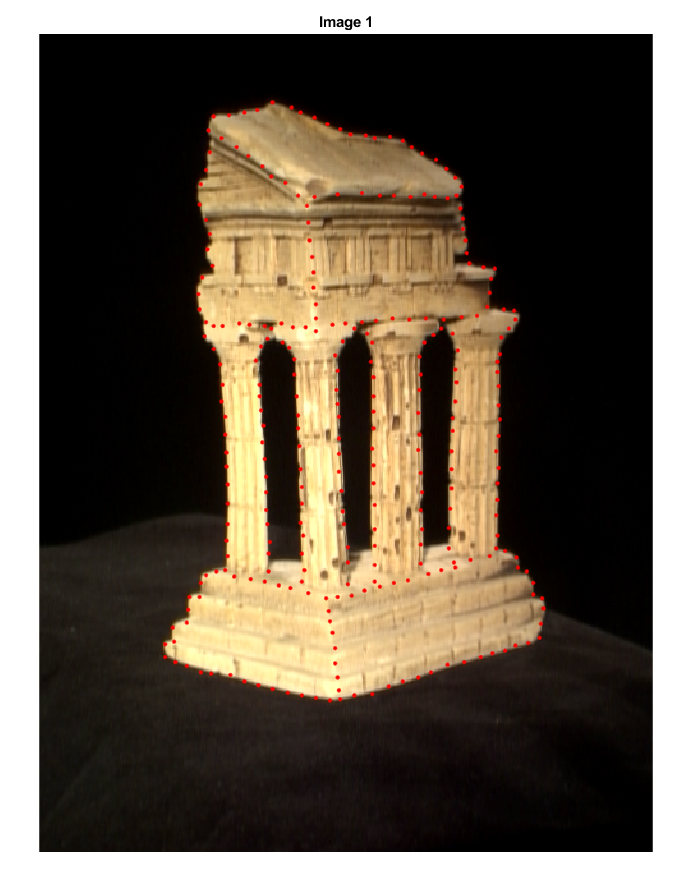
\includegraphics[width=1.2in]{Images/epipolarCorrespondeces1.png}}
        \qquad
        \subfloat[Correspondências obtidas]{\label{fig:8}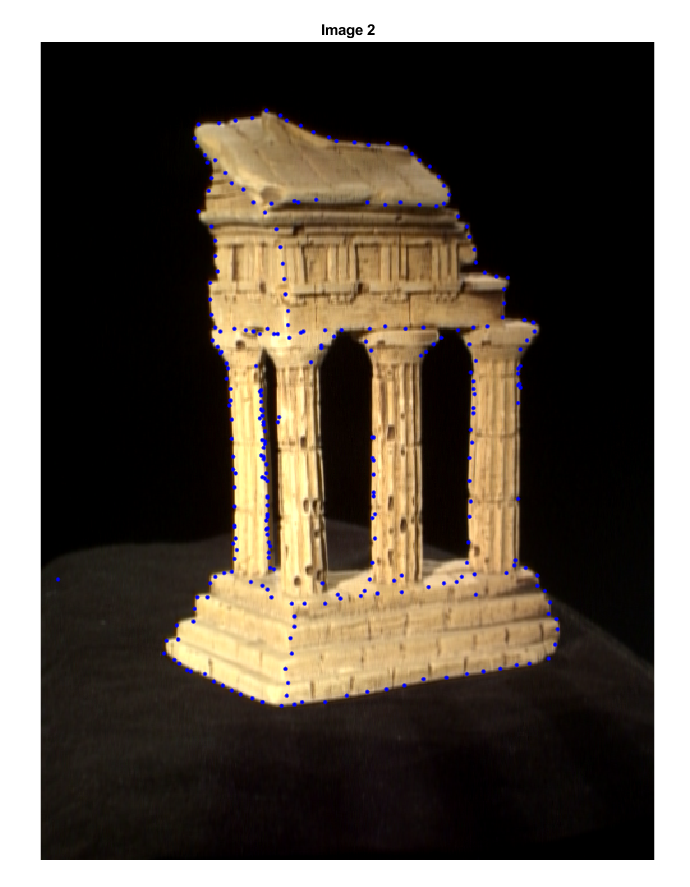
\includegraphics[width=1.2in]{Images/epipolarCorrespondeces2.png}}
        \caption{Correspondências epipolares}
        \label{fig:9}
\end{figure}
    
\subsection*{Matriz Essencial}
\par A estimação da matriz essencial é bastante simples, pois sendo conhecida a matriz fundamental e as matrizes intrínsecas da câmara, fornecidas pelo professor, basta aplicar a seguinte equação:
\begin{equation}
    E = K_2^TFK_1
\end{equation}
sendo $K_1$ e $K_2$ as matrizes intrínsecas da câmara para as respectivas imagens.
\par A matriz obtida por nós foi a seguinte:
\begin{equation}
    E =
    \begin{bmatrix}
    -0.0061 & -2.9674 & -0.2493 \\
    -0.8868 & 0.1087 & 14.8017 \\
    -0.1051 & -14.9963 & -0.0171
    \end{bmatrix}
\end{equation}

\subsection*{Estrutura 3D esparsa}
\par Para a estimação dos pontos 3D foi implementada uma função denominada \textit{triangulation}, esta vai ter como parâmetros de entrada os pontos da imagem da direita e os seus pontos correspondentes na imagem da esquerda e as matrizes de projeção de ambas as imagens.
\par Como consideramos que o eixo do mundo e da câmara 1 estão alinhados a sua matriz de projeção é simples de calcular.
\begin{equation}
    P_1 = K_1[I | 0]
\end{equation}
sendo $K_1$ a matriz dos parâmetros extrínsecos da câmara 1.
\par Para o cálculo da matriz de projeção da câmara 2 foi utilizada a função \textit{camera2} fornecida pelo professor. No entanto, esta função vai nos retornar as quatro possibilidades para a matriz de projeção.
\par A estrutura 3D vai ser calculada para as quatro possibilidades escolhendo depois aquela que produz uma estrutura 3D que esteja em frente a ambas as câmaras.
\par Para estimação dos pontos 3D vamos concatenar os pontos 2D de ambas as imagens e vamos resolver o seguinte sistema de equações lineares homogéneas:
\begin{equation}
    \begin{bmatrix}
    yp_3^T - p_2^T \\
    p_1^T - xp_3^T \\
    y'p_3'^T - p_2'^T \\
    p_1'^T - x'p_3'^T
    \end{bmatrix}
    X = 
    \begin{bmatrix}
    0 \\ 0 \\ 0 \\ 0
    \end{bmatrix}
\end{equation}
\par sendo $p_i, i=1,..,3$ a respectiva coluna da matriz de projecção da câmara 1, $p'_i, i=1,..,3$ da câmara 2 e $(x,y)$ $(x',y')$ o par de pontos correspondentes das imagens.
\par Para o cálculo deste sistema de equações foi feita a decomposição em valores singulares da primeira matriz.
\par Os resultados da nossa implementação do algoritmo de triangulação estão visualizados em baixo.

\begin{figure}[H]
        \centering
        \subfloat[]{\label{fig:10}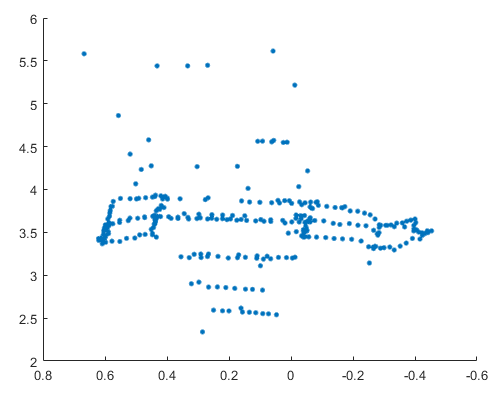
\includegraphics[width=1.2in]{Images/triang1.png}}
        \qquad
        \subfloat[]{\label{fig:11}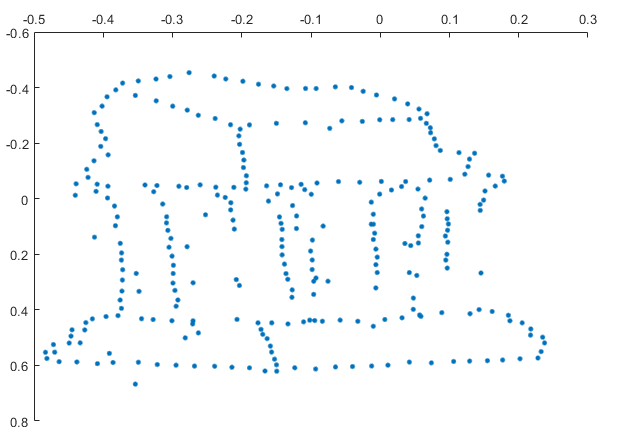
\includegraphics[width=1.2in]{Images/triang2.png}}
        \caption{Triangulação}
        \label{fig:12}
\end{figure}

\section{Dense Reconstruction}

\subsection*{Imagem Rectificada}
\par O primeiro passo para a reconstrução densa é rectificar as imagens da esquerda e da direita. O processo de rectificação consiste na transformação das imagens para que estas se apresentem no mesmo plano.
\par Ao rectificar as imagens vai facilitar bastante a correspondência de pontos entre duas imagens pois vai restringir o espaço de procura. Com as imagens rectificadas apenas vamos variando a coluna do pixel que estamos a comparar na imagem 2.
\par A função \textit{rectifyMatrices.m} retorna as matrizes M1 e M2 que são as matrizes de rectificação da imagem 1 e da imagem 2 respectivamente.
\begin{lstlisting}[
  caption=Calculo das transformações de rectificação,
  label=lst1:mxm,
  basicstyle=\small
]
%Computes the optical center
c1n=-inv(K1*R1)*K1*t1;
c2n=-inv(K2*R2)*K2*t2;

%Computes new Rotation Matrix
r1=(c1n-c2n)/norm(c1n-c2n);
r2=cross(R1(3,:)',r1);
r3=cross(r1,r2);

R1n=[r1'; r2'/norm(r2); r3'/norm(r3)];
R2n=R1n;

%Compute the new intrinsic parameters matrix
K1n=K2;
K2n=K2;

%Compute the new translation vectors
t1n=-R1n*c1n;
t2n=-R2n*c2n;

Compute the rectification matrices
M1=K1n*R1n*inv(K1*R1);
M2=K2n*R2n*inv(K2*R2);
\end{lstlisting}
\par Podemos ver na Fig.\ref{fig:4} que as linhas epipolares agora são totalmente horizontais como pretendido.
\begin{figure}[H]
    \centering
    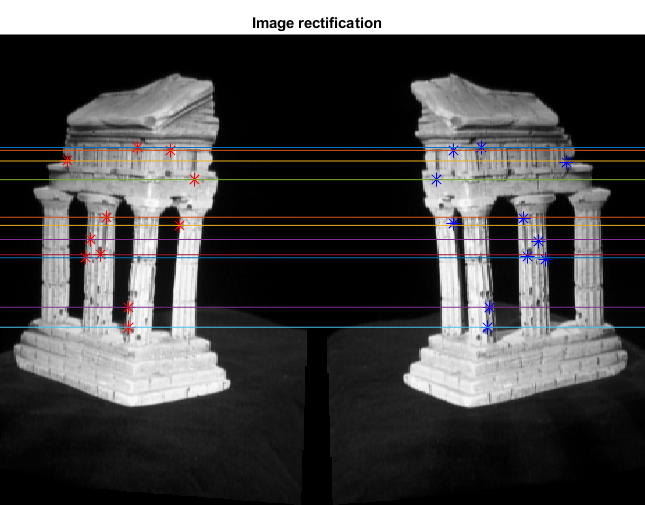
\includegraphics[width=2.5in]{Images/rectificationImages.png}
    \caption{Imagens retificadas}
    \label{fig:4}
\end{figure}
\subsection*{Mapa de Disparidade}
\par Disparidade é a distância entre a posição de dois pontos, o que nós vamos fazer é a estimação deste mapa. Onde uma cor branca mais acentuada significa que estão mais perto e uma cor mais escura que estão mais longe.
\par Para esta estimação foi implementada a função \textit{computeDisparity}, esta vai receber as duas imagens rectificadas, um valor máximo para a disparidade e tamanho do patch descritor.
\par O primeiro passo da nossa implementação vai ser encontrar todos os descritores para cada pixel da imagem 1,para tal, foi usada uma função desenvolvida num trabalho anterior denominada \textit{SimpleFeatureDescriptor}, para otimizar a nossa função foram apenas considerados pixeis não nulos, ignorando o fundo preto.
\par Como ambas as imagens estão retificadas a procura dos respectivos descritores na imagem 2 pode ser feita através de uma pesquisa horizontal.
\begin{equation}
    dispM(y,x) = \argmin_{-maxDisp\leq d \leq maxDisp} dist(im_1(y,x),im_2(y,x-d))
\end{equation}

\begin{lstlisting}[
  caption=Disparity Matrix,
  label=lst1:mxm,
  basicstyle=\tiny
]
for i=1:size(pts1,1)
        p2 = [];
        lowLimitX = max([pts1(i,1)-maxDisp 1]);
        highLimitX = min([pts1(i,1)+maxDisp size(im1,2)]);
        p2(:,1) = lowLimitX:highLimitX;
        p2(:,2) = y(i);
        
        %Gets all the descriptors for the points in the line
        [DesciptorsImg2]=SimpleFeatureDescriptor(im2,p2,windowSize); 
        %Matches the two descriptor
        [Match,~]=SSDFeatureMatching(DesciptorsImg1(i,:),DesciptorsImg2,10); 
        
         aux = min(Match(1,2:end-1));
         d = pts1(i,1) - p2(aux,1);
         dispM(y(i),x(i)) = abs(d);
end
\end{lstlisting}

\begin{figure}[H]
    \centering
    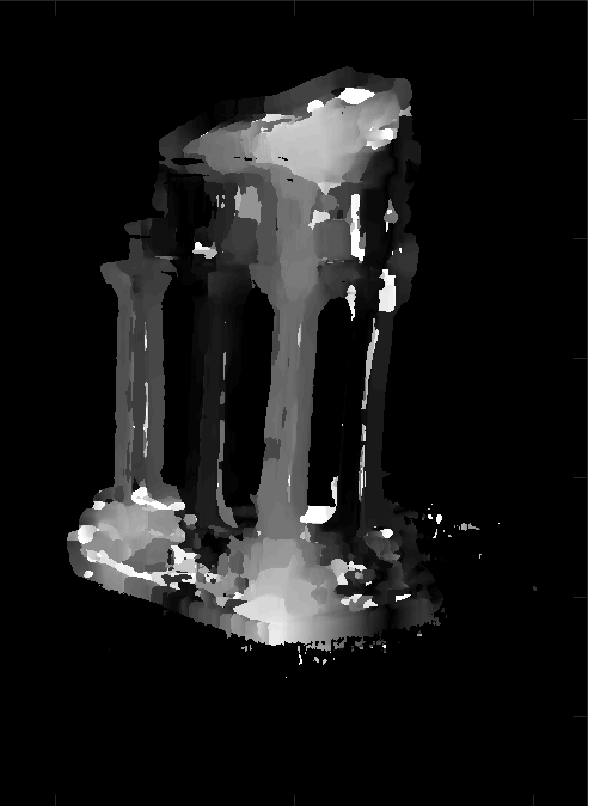
\includegraphics[width=2in]{Images/dMap.png}
    \caption{Mapa de Disparidade}
\end{figure}

\subsection*{Mapa de Profundidade}
\par Conhecendo a matriz de disparidade podemos agora estimar a profundidade para cada pixel através da seguinte equação:
\begin{equation}
    depthM(y,x) = \frac{b f}{dispM(y,x)}
\end{equation}
sendo $b$ a distância entre os centros ópticos e $f=K_1(1,1)$. Para os pixeis onde a disparidade é zero a profundidade também deve ser.
\begin{figure}[H]
    \centering
    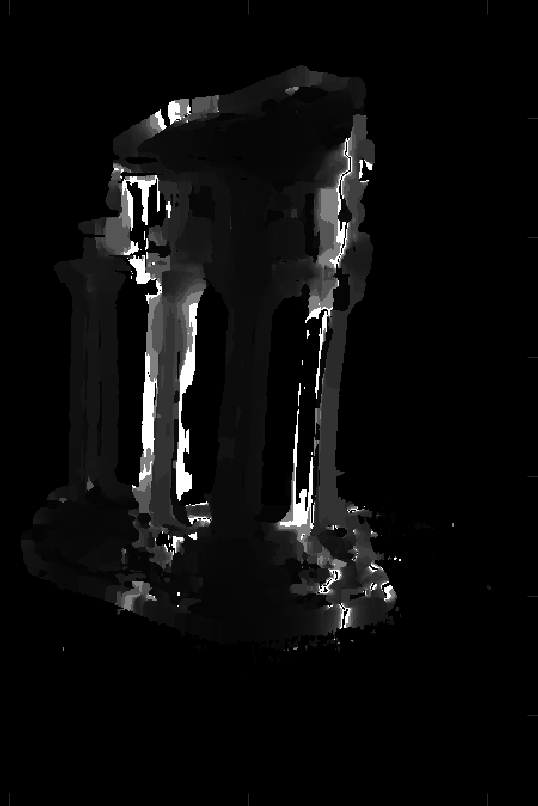
\includegraphics[width=2in]{Images/depMap.png}
    \caption{Mapa de Profundidade}
\end{figure}
\section{Conclusão}
\par Em conclusão, analisando os resultados apresentados, vemos que os algoritmos apresentados para a reconstrução esparsa e densa tiveram o comportamento esperado. Observamos também que o dimensionamento da janela do descritor SIMPLE tem uma grande influencia no funcionamento dos algoritmos, nomeadamente na correspondência entre as imagens.


\end{document}
